\section{MUMPS: Process Pinning}
\label{subseq:mm-mumps-process-pinning}

Due to intensive and complex manipulations with frontal and and contribution matrices, we can assume that MUMPS belongs to memory bound applications. In this case memory access can be a bottleneck for the library. A common way to improve performance of memory bound applications running on distributed memory machines is to distribute processes equally among NUMA domains within a compute node. Given the fact that each NUMA domain has its own system bus, this strategy allows to reduce conjunction of memory traffic by balancing data requests equally among the memory channels.\\


However, because MUMPS uses both task and data parallelism as well as a complex hybrid, both static and dynamic, task scheduling, it becomes difficult to decide which pinning strategy is better i.e. \textit{close} or \textit{spread}, described in section \ref{subseq:matrix-sets-and-hardware}.\\


Therefore, a couple of tests were conducted with both GRS and SuiteSparse matrix sets in order to investigate influence of different strategies on MUMPS performance. For this group of tests, MUMPS was used with default settings and a specific fill-in reducing algorithm for each test case, mentioned in section \ref{subseq:fill-in-reordering}. The tests were performed on both HW1 and HW2 machines using only flat-MPI mode. This comparison allows to investigate influence of number independent system buses of a compute node on MUMPS overall performance since HW1 and HW2 machines have different number of NUMA domains, 2 and 4, respectively. Results are shown in figures \ref{fig:mumps-close-vs-spread-1}, \ref{fig:mumps-close-vs-spread-2}, \ref{fig:mumps-close-vs-spread-3} and in appendix \ref{app:mm-mumps-process-pinning}. The graphs depict the total time of MUMPS, i.e. time spent on analysis, factorization and solution phases.\\

\figpointer{\ref{fig:mumps-close-vs-spread-1}}
\begin{figure}[htpb]
\centering
	\begin{tabular}{cc}
	\subfloat[HW1 - pwr-3d]{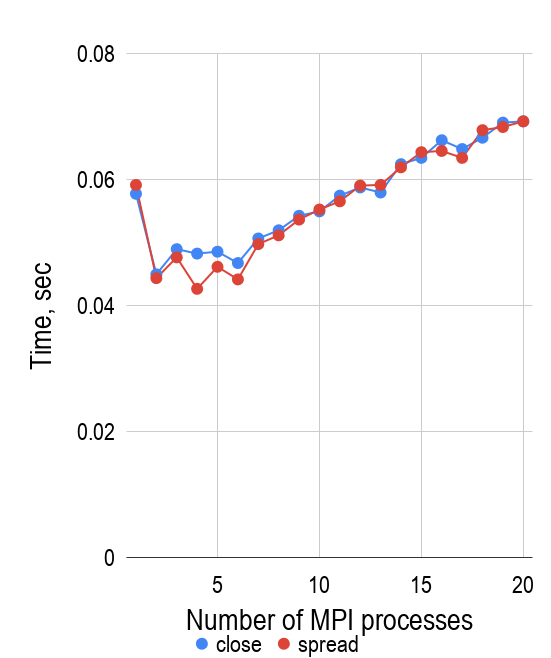
\includegraphics[width=0.48\textwidth]{figures/chapter-2/spread-vs-close/grs-cluster/pwr-3d.png}} &
		\subfloat[HW2 - pwr-3d]{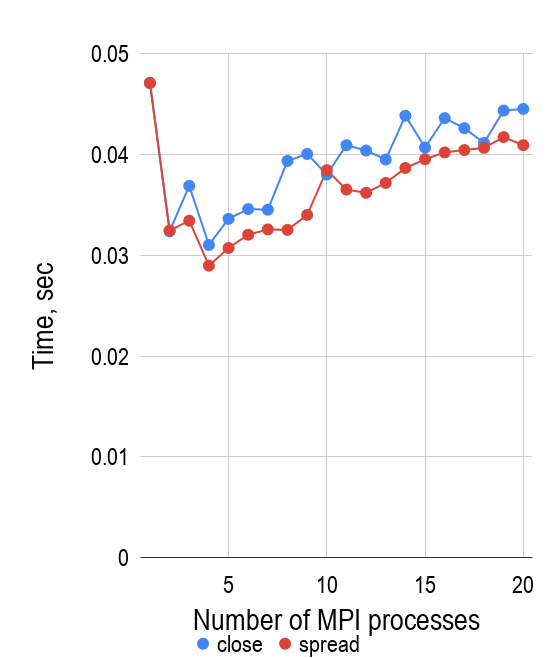
\includegraphics[width=0.48\textwidth]{figures/chapter-2/spread-vs-close/linux-cluster/pwr-3d.png}} \\
		\subfloat[HW1 - cube-64]{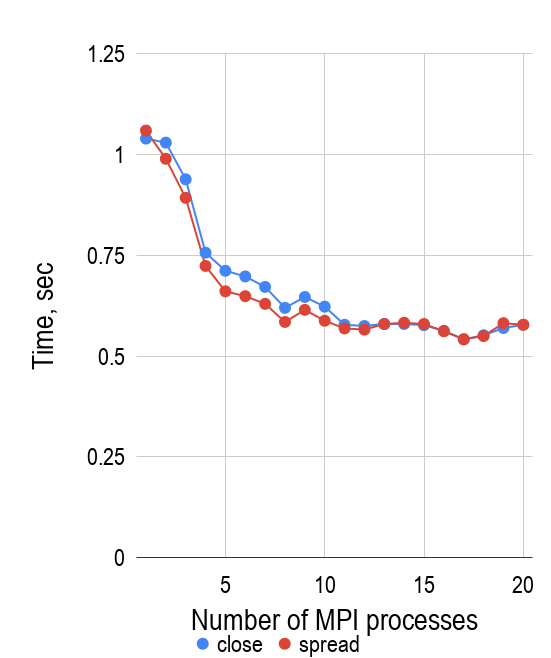
\includegraphics[width=0.48\textwidth]{figures/chapter-2/spread-vs-close/grs-cluster/cube-64.png}} &
		\subfloat[HW2 - cube-64]{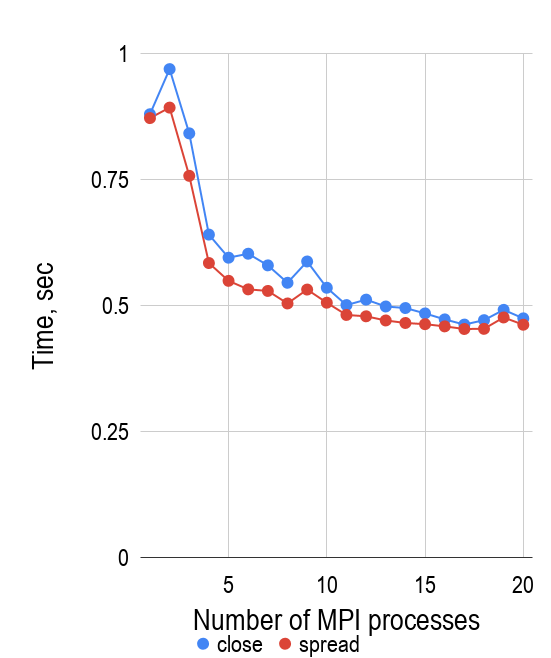
\includegraphics[width=0.48\textwidth]{figures/chapter-2/spread-vs-close/linux-cluster/cube-64.png}} \\
	\end{tabular}
	\caption{Comparison of \textit{close} and \textit{spread} pinning strategies}
	\label{fig:mumps-close-vs-spread-1}
\end{figure}



\figpointer{\ref{fig:mumps-close-vs-spread-2}}
\begin{figure}[htpb]
\centering
	\begin{tabular}{cc}
		\subfloat[HW1 - cube-645]{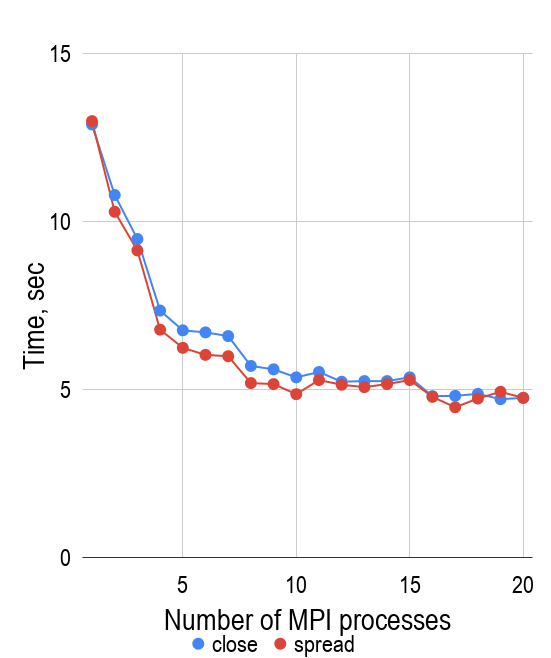
\includegraphics[width=0.48\textwidth]{figures/chapter-2/spread-vs-close/grs-cluster/cube-645.png}} &
		\subfloat[HW2 - cube-645]{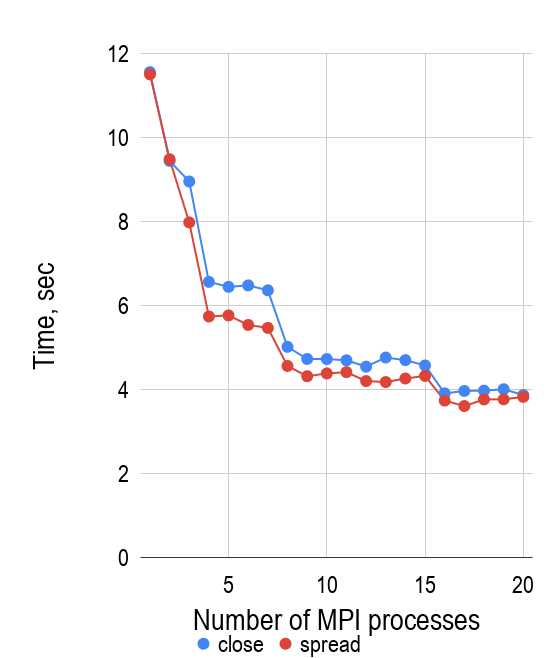
\includegraphics[width=0.48\textwidth]{figures/chapter-2/spread-vs-close/linux-cluster/cube-645.png}} \\
		\subfloat[HW1 - k3-18]{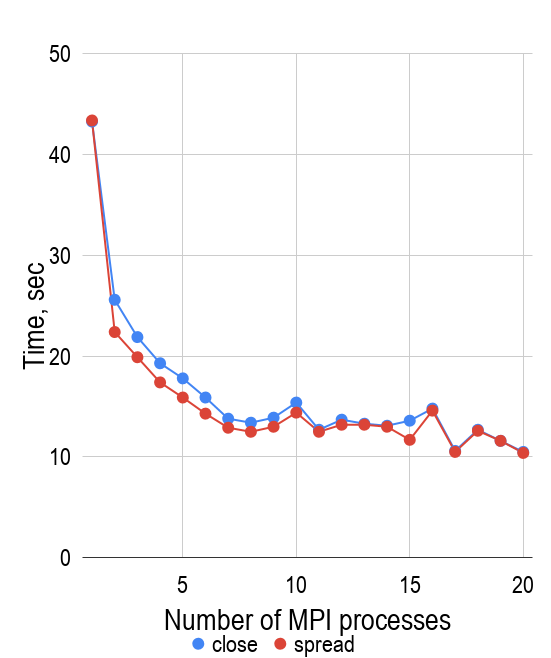
\includegraphics[width=0.48\textwidth]{figures/chapter-2/spread-vs-close/grs-cluster/k3-18.png}} &
		\subfloat[HW2 - k3-18]{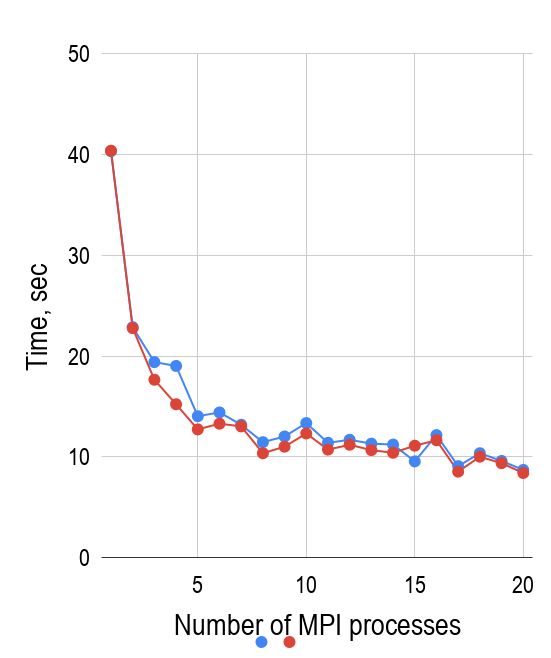
\includegraphics[width=0.48\textwidth]{figures/chapter-2/spread-vs-close/linux-cluster/k3-18.png}} \\
	\end{tabular}
	\caption{Comparison of \textit{close} and \textit{spread} pinning strategies}
	\label{fig:mumps-close-vs-spread-2}
\end{figure}




\figpointer{\ref{fig:mumps-close-vs-spread-3}}
\begin{figure}[htpb]
\centering
	\begin{tabular}{cc}
		\subfloat[HW1 - PFlow\_742]{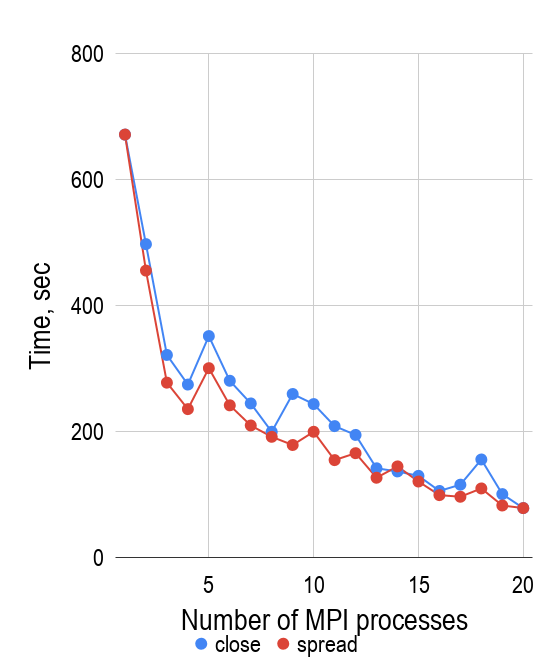
\includegraphics[width=0.48\textwidth]{figures/chapter-2/spread-vs-close/grs-cluster/PFlow_742.png}} &
		\subfloat[HW2 - PFlow\_742]{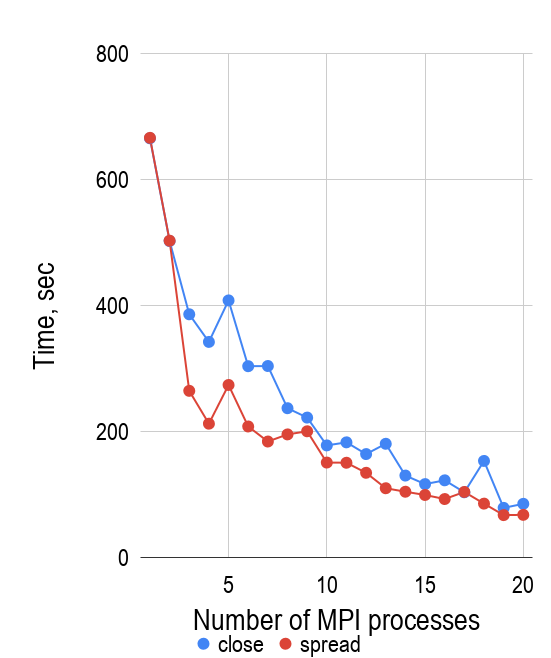
\includegraphics[width=0.48\textwidth]{figures/chapter-2/spread-vs-close/linux-cluster/PFlow_742.png}} \\
		\subfloat[HW1 - CurlCurl\_3]{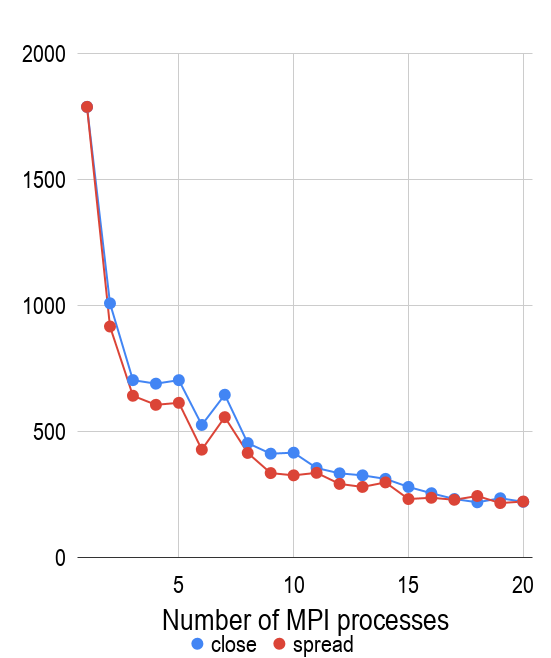
\includegraphics[width=0.48\textwidth]{figures/chapter-2/spread-vs-close/grs-cluster/CurlCurl_3.png}} &
		\subfloat[HW2 - CurlCurl\_3]{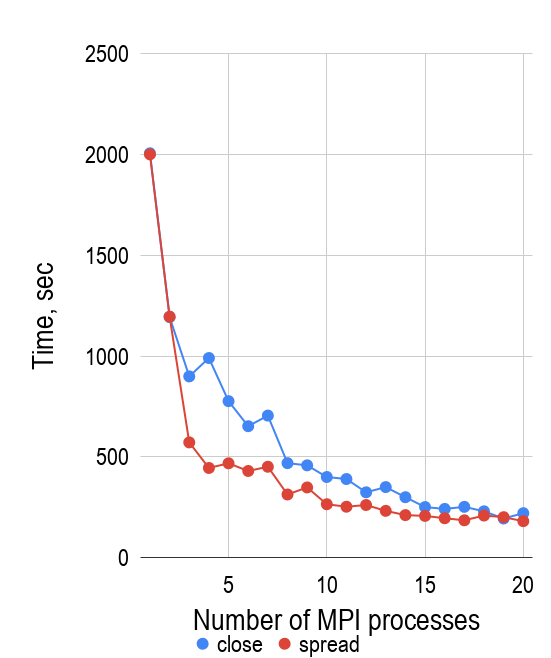
\includegraphics[width=0.48\textwidth]{figures/chapter-2/spread-vs-close/linux-cluster/CurlCurl_3.png}} \\
	\end{tabular}
	\caption{Comparison of \textit{close} and \textit{spread} pinning strategies}
	\label{fig:mumps-close-vs-spread-3}
\end{figure}


The tests revealed that, in general, \textit{spread}-pinning performed better on both machines. In average, the strategy allows to reduce run-time by approximately 5.5\% and 13.8\% on HW1 and HW2 machines, respectively. The main performance gain can be observed in the middle range of process count i.e. the range from 2 to 12, where the view on the process distribution, between \textit{close} and \textit{spread} strategies, varies considerably. On another hand, the performance gain becomes less prominent while moving towards the tail of process count since difference of process distribution becomes negligible. As expected for HW1, the points where process count is equal to 1 and 20 show the same performance because they basically represent the same process distribution.\\


It is also important to investigate the gain of performance around the saturation point. It is worth pointing out that from time to time it becomes very difficult to decide where the saturation point locates. For that reason, a careful analysis was performed for each graph based on values of speed-up, efficiency and our subjective opinion. The results are summarized in tables \ref{table:pinning-comparison-grs-matrix-set} and \ref{table:pinning-comparison-suitesparse-matrix-set}. \\


\begin{table}[htpb]
\centering
\small
\begin{tabular}{c|c|c|c|c|c|c|c|c|c|}
\cline{2-5} \cline{7-10}
                                                                            & \multicolumn{4}{c|}{HW1}                                                                                                                                                                  &  & \multicolumn{4}{c|}{HW2}                                                                                                                                                                  \\ \cline{1-5} \cline{7-10} 
\multicolumn{1}{|c|}{\begin{tabular}[c]{@{}c@{}}Matrix\\ Name\end{tabular}} & MPI & \begin{tabular}[c]{@{}c@{}}Gain\\ w.r.t\\ "close", \\ \%\end{tabular} & \begin{tabular}[c]{@{}c@{}}Speed\\ up\end{tabular} & \begin{tabular}[c]{@{}c@{}}Effi-\\ ciency\end{tabular} &  & MPI & \begin{tabular}[c]{@{}c@{}}Gain\\ w.r.t\\ "close", \\ \%\end{tabular} & \begin{tabular}[c]{@{}c@{}}Speed\\ up\end{tabular} & \begin{tabular}[c]{@{}c@{}}Effi-\\ ciency\end{tabular} \\ \cline{1-5} \cline{7-10} 
\multicolumn{1}{|c|}{pwr-3d}                                                & 4   & 11.594                                                             & 1.386                                              & 0.347                                                  & \multicolumn{1}{c|}{} & 4   & 6.616                                                              & 1.626                                              & 0.406                                                  \\ \cline{1-5} \cline{7-10} 
\multicolumn{1}{|c|}{cube-5}                                                & 4   & 8.261                                                              & 1.139                                              & 0.285                                                  & \multicolumn{1}{c|}{} & 4   & 10.640                                                             & 1.156                                              & 0.289                                                  \\ \cline{1-5} \cline{7-10} 
\multicolumn{1}{|c|}{cube-64}                                               & 8   & 5.645                                                              & 1.812                                              & 0.226                                                  & \multicolumn{1}{c|}{} & 8   & 7.521                                                              & 1.729                                              & 0.216                                                  \\ \cline{1-5} \cline{7-10} 
\multicolumn{1}{|c|}{cube-645}                                              & 6   & 9.985                                                              & 2.152                                              & 0.359                                                  & \multicolumn{1}{c|}{} & 8   & 9.078                                                              & 2.521                                              & 0.315                                                  \\ \cline{1-5} \cline{7-10} 
\multicolumn{1}{|c|}{k3-2}                                                  & 7   & 7.788                                                              & 2.899                                              & 0.414                                                  & \multicolumn{1}{c|}{} & 8   & 9.947                                                              & 3.298                                              & 0.412                                                  \\ \cline{1-5} \cline{7-10} 
\multicolumn{1}{|c|}{k3-18}                                                 & 8   & 6.716                                                              & 3.472                                              & 0.434                                                  & \multicolumn{1}{c|}{} & 8   & 9.567                                                              & 3.896                                              & 0.487                                                  \\ \cline{1-5} \cline{7-10} 
\end{tabular}
\caption{Analysis and comparison of MUMPS performance at the saturation point between HW1 and HW2 for GRS matrix set}
\label{table:pinning-comparison-grs-matrix-set}
\end{table}



\begin{table}[htpb]
\centering
\small
\begin{tabular}{c|c|c|c|c|c|c|c|c|c|}
\cline{2-5} \cline{7-10}
                                                                            & \multicolumn{4}{c|}{HW1}                                                                                                                                                                  &  & \multicolumn{4}{c|}{HW2}                                                                                                                                                                  \\ \cline{1-5} \cline{7-10} 
\multicolumn{1}{|c|}{\begin{tabular}[c]{@{}c@{}}Matrix\\ Name\end{tabular}} & MPI & \begin{tabular}[c]{@{}c@{}}Gain\\ w.r.t\\ "close", \\ \%\end{tabular} & \begin{tabular}[c]{@{}c@{}}Speed\\ up\end{tabular} & \begin{tabular}[c]{@{}c@{}}Effi-\\ ciency\end{tabular} &  & MPI & \begin{tabular}[c]{@{}c@{}}Gain\\ w.r.t\\ "close", \\ \%\end{tabular} & \begin{tabular}[c]{@{}c@{}}Speed\\ up\end{tabular} & \begin{tabular}[c]{@{}c@{}}Effi-\\ ciency\end{tabular} \\ \cline{1-5} \cline{7-10} 
\multicolumn{1}{|c|}{cant}                                                  & 8   & 7.914                                                                 & 3.297                                              & 0.412                                                  &  & 8   & 12.437                                                                & 3.407                                              & 0.426                                                  \\ \cline{1-5} \cline{7-10} 
\multicolumn{1}{|c|}{consph}                                                & 15  & 0.110                                                                 & 6.147                                              & 0.410                                                  &  & 15  & 2.409                                                                 & 6.667                                              & 0.444                                                  \\ \cline{1-5} \cline{7-10} 
\multicolumn{1}{|c|}{CurlCurl\_3}                                           & 19  & 8.051                                                                 & 8.249                                              & 0.434                                                  &  & 20  & 17.908                                                                & 11.039                                             & 0.552                                                  \\ \cline{1-5} \cline{7-10} 
\multicolumn{1}{|c|}{Geo\_1438}                                             & 13  & 21.609                                                                & 4.548                                              & 0.350                                                  &  & ROM & ROM                                                                   & ROM                                                & ROM                                                    \\ \cline{1-5} \cline{7-10} 
\multicolumn{1}{|c|}{memchip}                                               & 9   & 11.290                                                                & 4.299                                              & 0.477                                                  &  & 9   & 11.102                                                                & 4.213                                              & 0.468                                                  \\ \cline{1-5} \cline{7-10} 
\multicolumn{1}{|c|}{PFlow\_742}                                            & 19  & 17.921                                                                & 8.106                                              & 0.427                                                  &  & 20  & 20.469                                                                & 9.798                                              & 0.490                                                  \\ \cline{1-5} \cline{7-10} 
\multicolumn{1}{|c|}{pkustk10}                                              & 17  & -0.664                                                                & 3.872                                              & 0.228                                                  &  & 17  & -1.108                                                                & 4.036                                              & 0.237                                                  \\ \cline{1-5} \cline{7-10} 
\multicolumn{1}{|c|}{torso3}                                                & 18  & 5.607                                                                 & 8.149                                              & 0.453                                                  &  & 19  & 6.028                                                                 & 9.493                                              & 0.499                                                  \\ \cline{1-5} \cline{7-10} 
\multicolumn{1}{|c|}{x104}                                                  & 6   & 9.537                                                                 & 1.789                                              & 0.298                                                  &  & 6   & 7.829                                                                 & 1.763                                              & 0.294                                                  \\ \cline{1-5} \cline{7-10} 
\end{tabular}
\caption{Analysis and comparison of MUMPS performance at the saturation point between HW1 and HW2 for SuiteSparse matrix set.\\
*ROM - run out of memory}
\label{table:pinning-comparison-suitesparse-matrix-set}
\end{table}


% comparison of different machines
A study of tables \ref{table:pinning-comparison-grs-matrix-set} and \ref{table:pinning-comparison-grs-matrix-set} reveals HW2 machine performs slightly better in contrast to HW1 with respect to performance gain around the saturation points. This result is considerably different from the overall performance gain that was mentioned above where the difference was as twice as much. However, the results also show that increase of NUMA domains always help to improve the values of efficiency and speed-up and thus strong scaling behavior of MUMPS.\\

% Conclusion: process distribution can help in case of energy save computing

In this section, we showed influence of process distribution as well as the NUMA domain count on overall MUMPS parallel performance. We show the \textit{spread} process distribution always has some beneficial effect. The increase of NUMA domains also brings some extra performance but not too much as it was expected at the beginning.\\ 


This result of this study can be relevant for energy efficient parallel computing where a strong requirements to program efficiency are applied. This fact usually forces the user to decrease process count and go a slightly away from saturation point in order to keep the values of efficiency around 0.7-0.8. In this case performance of MUMPS can be improved in 15-20\% in contrast to the straight forward process pinning.\\


Taken into account results of the tests, \textit{spread}-pinning has been chosen for the rest of the study. This process distribution can be easily achieved by means of some advanced OpenMPI command line options, for example \textit{--rank-by} and \textit{--bind-to}, as following:. \\

\begin{lstlisting}[language=bash, caption={An example of \textit{spread}-pinning with using  advanced OpenMPI command line options}, frame=single, label={lst:iterative-refinement}]
mpiexec --rank-by numa --bind-to core -n $num_proc $executable_name $parameters
\end{lstlisting}
